\subsection{Nobreaks} \label{section: nobreak}
TEXTO A SER ESCRITO

\subsubsection{Generalidades}
\begin{enumerate}
	\item Quando o projeto de distribuição elétrica exigir, deverá ser previsto a utilização de sistema de nobreak’s que sejam compatíveis e, possibilitem serem alimentados a partir dos grupos motor geradores de emergência (GMGs) a serem instalados no sistema. 
	
	\item Os nobreak’s deverão possuir conjuntos de baterias que possibilitem uma autonomia mínima de 15 minutos para todo o sistema de energia estabilizada.
	
	\item Os nobreak’s projetados deverão possuir obrigatoriamente entrada trifásica e saída trifásica. Casos excepcionais, a contratada deverá ser consultada.
	
	\item Sempre deverá ser previsto um sistema de by-pass, de modo que em caso de manutenção ou problemas operacionais o ramal de alimentação das cargas estará sempre em linha;
	
	\item Alguns equipamentos necessitam estar ligados a energia ininterrupta:
	\begin{table}[ht]
		\rowcolors{2}{Tue-red!10}{white}
		\centering
		\caption{Equipamentos obrigatórios no nobreak}
		\begin{tabular}[t]{ccc}
			\toprule
			\color{Tue-red}\textbf{Equipamento}&\color{Tue-red}\textbf{Pot. mínima}&\color{Tue-red}\textbf{Pot. máxima}\\
			\midrule
			XXXXX&0W&0W\\
			XXXXX&0W&0W\\
			XXXXX&0W&0W\\
			XXXXX&0W&0W\\
			\bottomrule
		\end{tabular}
		\label{table: equipamentosxnobreak}
	\end{table}
	
	\item Condições específicas serão vistas posteriormente.
	
	\item Nos casos que se faça necessário o uso de redundância de \textit{nobreaks} e o contratante não estabeleça o tipo de redundância(\textit{BACKUP}) a ser empregado, caberá ao projetista propor o tipo de redundância a ser empregado (de acordo com o item \ref{nobreak: tipo de redundancia}) e obter aprovação do contratante.
	
	\item Possíveis redundâncias de nobreak's caso seja necessária.
	\begin{enumerate}\label{nobreak: tipo de redundancia}
		\item Redundância em cascata/\textit{by-pass}, figura \ref{fig: redundancia1}
		
		\item Paralelismo redundante, figura  \ref{fig: redundancia2}
		
		\item Paralelismo N + 1, figura  \ref{fig: redundancia3}
		
		\item Paralelismo modular, figura  \ref{fig: redundancia4}
		
		\item Outras indicadas pela contratada
		
	\end{enumerate}

	\begin{figure}[H]
		\centering
		\begin{minipage}{0.45\textwidth}
			\centering
			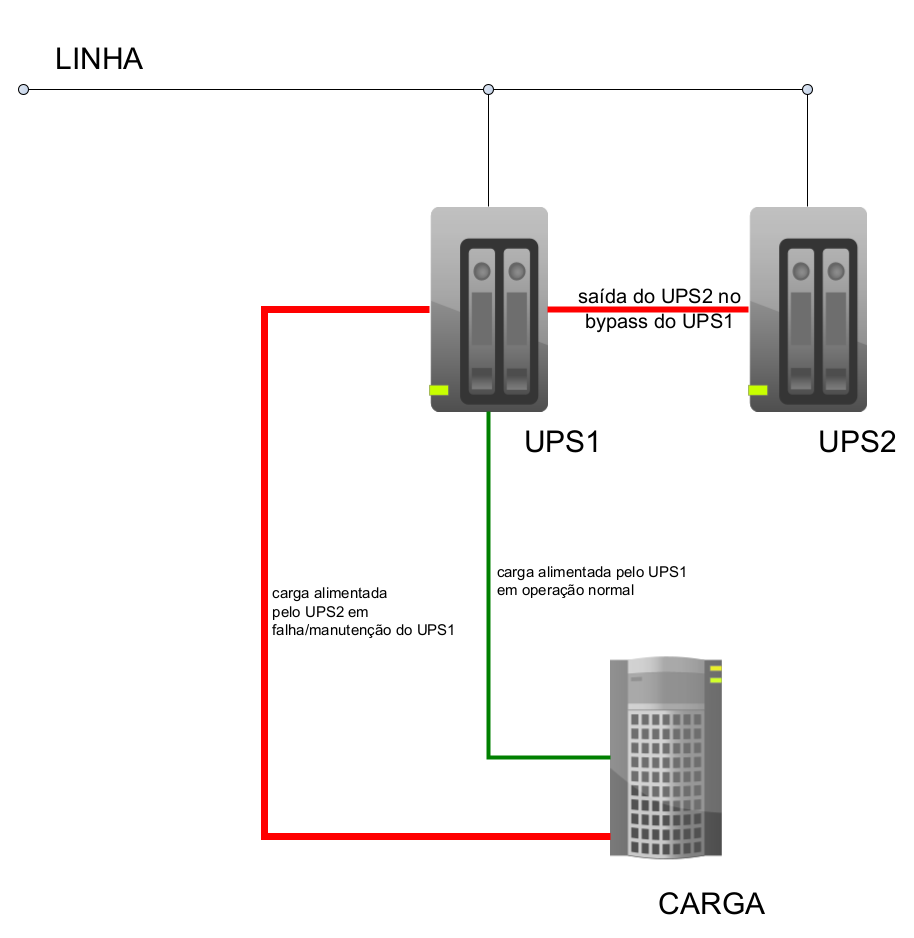
\includegraphics[width=\textwidth]{Figures/7. nobreak/redundancia1.png}
			\captionof{figure}{Redundância em cascata/by-pass}
			\label{fig: redundancia1}
		\end{minipage}
		\hfill
		\begin{minipage}{0.45\textwidth}
			\centering
			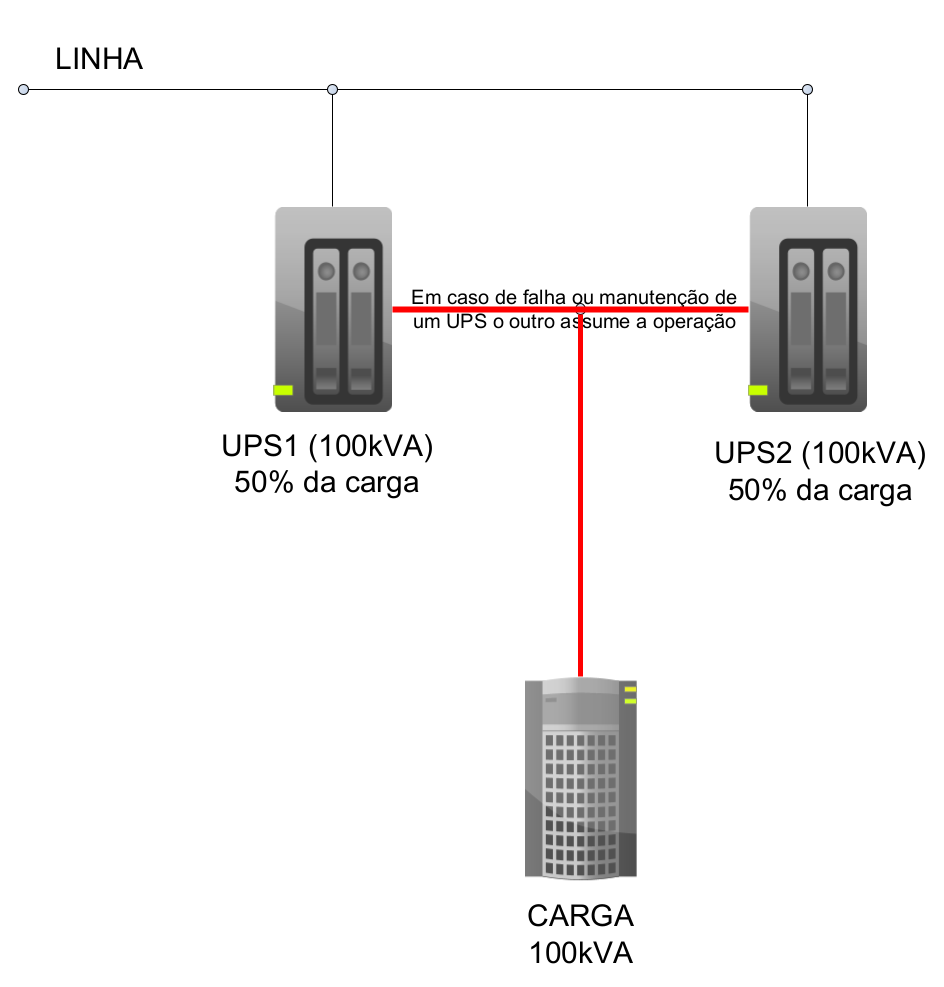
\includegraphics[width=\textwidth]{Figures/7. nobreak/redundancia2.png}
			\captionof{figure}{Paralelismo redundante}
			\label{fig: redundancia2}
		\end{minipage}
	\end{figure}
	\begin{figure}[H]
	\centering
		\begin{minipage}{0.45\textwidth}
			\centering
			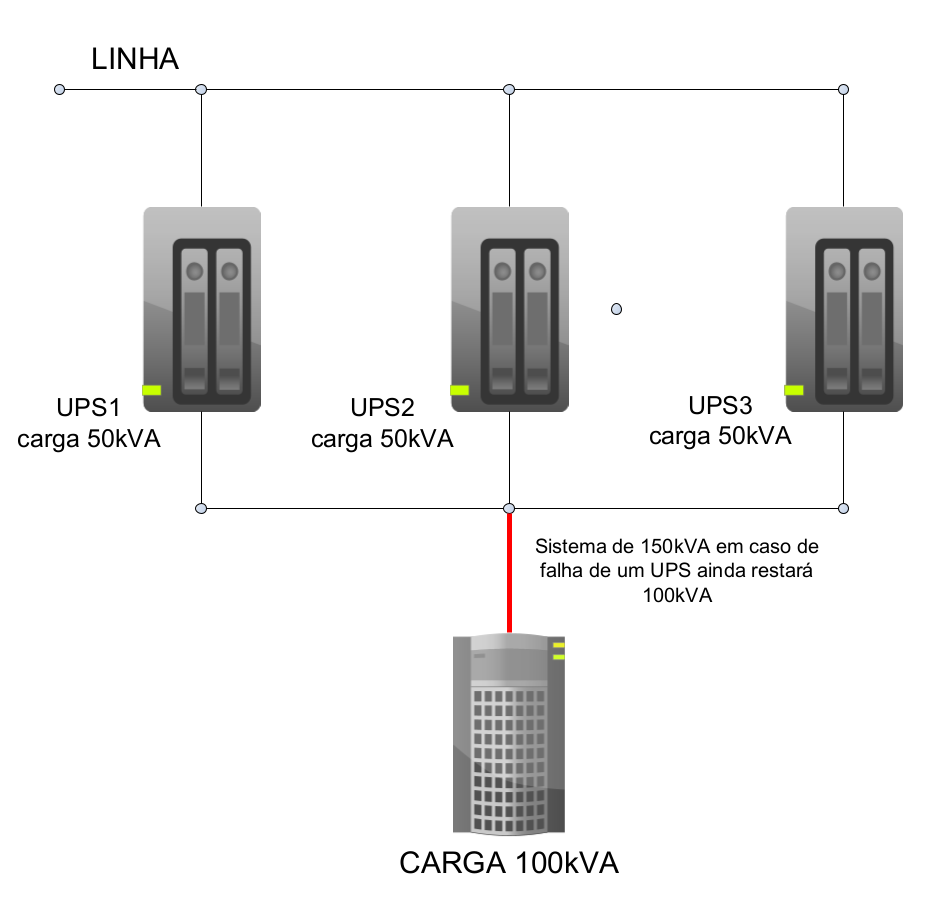
\includegraphics[width=\textwidth]{Figures/7. nobreak/redundancia3.png}
			\captionof{figure}{Paralelismo N + 1}
			\label{fig: redundancia3}
		\end{minipage}
		\begin{minipage}{0.45\textwidth}
			\centering
			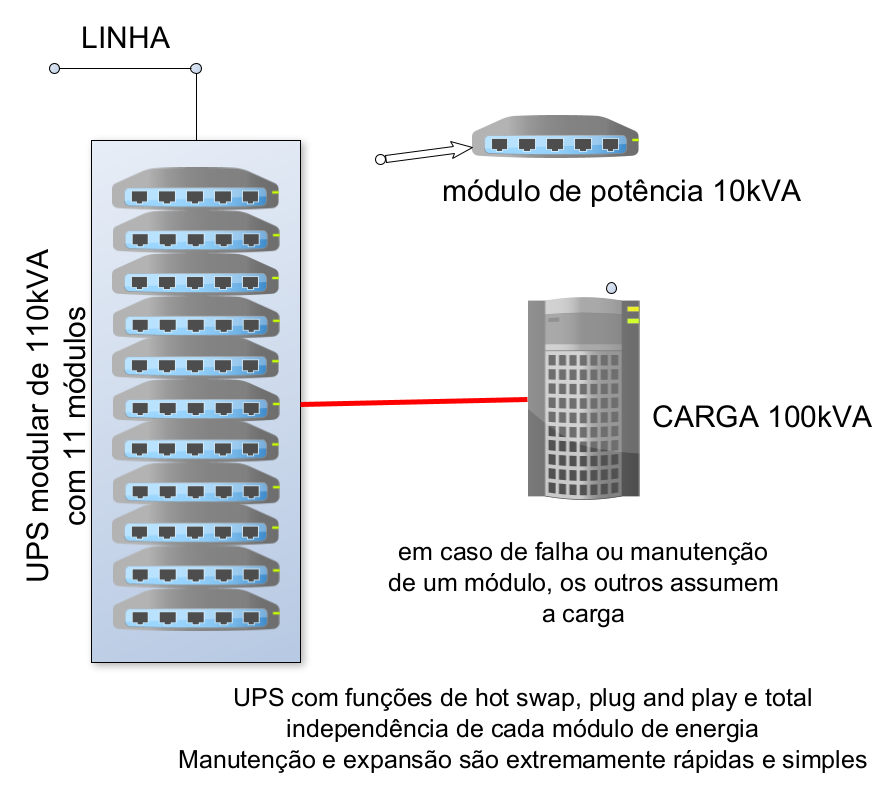
\includegraphics[width=\textwidth]{Figures/7. nobreak/redundancia4.png}
			\captionof{figure}{Paralelismo modular}
			\label{fig: redundancia4}
		\end{minipage}
	\end{figure}

\end{enumerate}